\chapter{Introduction}

\section{Background}

With the advent of computing, a large amount of data is being created
everyday~\cite{emc}.
Raw data exists in many forms --- numbers, texts, images, audio, video, etc.,
most of it unstructured or semi-structured~\cite{emc},
and requires processing in order to derive meaning. Of particular interest for
research purposes are multimedia data (audio and video), specifically
multimedia data of the following three prevalent types:

\begin{itemize}
    \item Single-file audio --- radio recordings, interviews and talk shows
    \item Single-file video --- televised news and speeches
    \item Multi-channel audio --- recorded conversations using multiple
    microphones
\end{itemize}

A general pipeline to process and index multimedia data would look like this:

\begin{figure}[h]
\begin{center}
    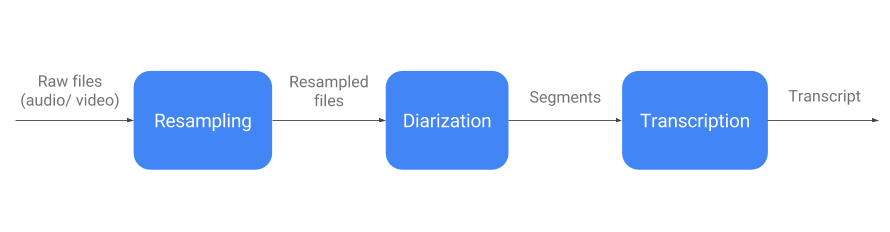
\includegraphics[width=\textwidth]{../images/pipeline.png}
    \caption{Multimedia processing pipeline}
\end{center}
\end{figure}

The multimedia files are first crawled from a source (website or database) by
means of a crawler, or created using recording instruments. These files would
then go through a pipeline of processing tasks to extract useful information
for indexing, storage and visualization. The data visualizations could be
indexed and stored together with the processing outputs. 

For multimedia data, a textual representation of the data is often desirable
as a precursor to further processing. Two processes are capable of converting
multimedia into text:

\begin{itemize}
    \item Transcription --- the process of converting speech to
    text~\cite{transcribe-mw}
    \item Captioning --- the process of converting image to description
    of such image~\cite{caption}
\end{itemize}

Transcription is a well-defined pipeline:

\begin{figure}[h]
\begin{center}
    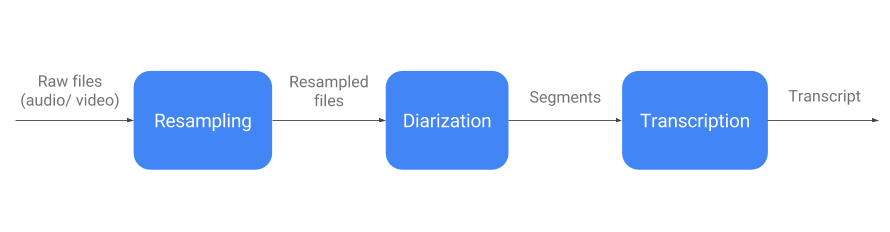
\includegraphics[width=\textwidth]{../images/pipeline_transcribe.png}
    \caption{Transcription processing pipeline}
\end{center}
\end{figure}

Transcription starts with the raw audio or video file, which could be
single-speaker (for example lecture recordings, Parliament speeches) or
multi-speaker (for example conversations, talk shows). The file is then resampled
to an appropriate configuration of bit rate and sample size. The resampled audio
goes through the process of speaker diarization, to separate different audio
segments (usually short) said by different speakers. These short segments are
then fed one-by-one to a transcription system; combining all the results gives
the final transcript.

For each process in the pipeline, there exists multiple solutions to perform
the task. Many of them are either public application programming interfaces (APIs)
or open-source; however, they exist as ``black boxes'' --- each solution accepts
input and produces output in a specific manner. This presents a challenge in
integrating multiple solutions to realise the transcription pipeline.
Additionally, given an integrated pipeline, upgrading or changing any component
could potentially break the pipeline. After the pipeline is upgraded, there must
also be a mechanism to update the transcriptions and keep track of versions. 

This project proposes an integrated transcription system; apart from realising
the transcription pipeline, this system would be able to accommodate versioning
of all the pipeline components as well as all the transcripts. Ultimately, this
results in a simple and more efficient processing workflow for multimedia.

This project would be done in conjunction with other efforts of the Speech and
Language Research Group at the School of Computer Science and Engineering (SLRG)
~\cite{slrg}.

\section{Objective}

The primary objective of this project is to design a system architecture and
develop the respective system capable of performing the following tasks:

\begin{itemize}
    \item Transcription of individual audio and video files using different
    transcription solutions
    \item Transcription of multi-channel audio recording
\end{itemize}

The developed system must also have the following qualitative requirements:

\begin{itemize}
    \item Modularity --- allowing independent component operation and low coupling
    \item Extensibility --- allowing system extension to perform other related
    tasks in audio and video processing
    \item Robustness --- allowing system error recovery and process resumption
    \item Versioning --- allowing for different results with different processing
    components, and enabling evaluation of different components
    \item Logging and Reporting --- allowing developers to understand and generate
    insights to the outputs
\end{itemize}

\section{Scope}

The scope of this project is restricted to developing a system to be used in a
desktop/ laptop Ubuntu Linux environment, to perform the tasks mentioned above. A
functioning graphics user interface (GUI) is also not required.

However, the system could be modified and extended to perform other related tasks
in different environments, with a GUI\@.

\section{Project Timeline}

The project was scheduled to commence from January 2017 to October 2017. The major
milestones are as follows:

\begin{itemize}
    \item \textbf{End of January 2017:} Completion of Architectural Design
    \item \textbf{End of April 2017:} Completion of Porting of Existing Modules
    to Current System
    \item \textbf{End of September 2017:} Completion of Development of New Modules;
    Commencement of Integration Testing
    \item \textbf{End of October 2017:} Completion of Project
    \item \textbf{End of December 2017:} Project Presentation and Handover
\end{itemize}

\section{Report Organisation}

This report is divided into four chapters:

\begin{itemize}
    \item Chapter 1 provides an introduction to the project, states its objective
    and scope and provides a timeline for completion.
    \item Chapter 2 gives a summary of the work done so far on the project
    \item Chapter 3 gives an overview to the remaining work to be done before the
    project completes.
    \item Chapter 4 concludes the report.
\end{itemize}